\documentclass[10pt]{beamer}
%
%   Arquivo de Configuração dos Slides
%


%
%   Pacotes utilizados
%

% Codificação dos caracteres em formato universal.
\usepackage[utf8]{inputenc}
\usepackage[T1]{fontenc}

% Traduz o texto gerados pelo LaTeX para português. ex.: Capítulo, Seção, Conteúdo.
\usepackage[brazil]{babel}

% Pacotes para ambientes matemáticos
\usepackage{amsmath}
\usepackage{amsthm}
\usepackage{amssymb}

% Diversas funções para o uso das aspas.
\usepackage{csquotes}

% Outros pacotes
\usepackage{hyperref}
\usepackage{tikz}
\usepackage{yfonts}
\usepackage{colortbl}
\usepackage{ragged2e}
\usepackage{helvet}
\usepackage{verbatim}


%
%   Tema
%

% Copyright 2007 by Till Tantau
%
% This file may be distributed and/or modified
%
% 1. under the LaTeX Project Public License and/or
% 2. under the GNU Public License.
%
% See the file doc/licenses/LICENSE for more details.


% Common packages


\usepackage[brazil]{babel}
\usepackage[utf8]{inputenc}
\usepackage{times}
 \mode<article> {
  \usepackage{times}
  \usepackage{mathptmx}
  \usepackage[left=1.5cm,right=6cm,top=1.5cm,bottom=3cm]{geometry}
}

\usepackage{hyperref}
\usepackage[T1]{fontenc}
\usepackage{amsmath,amssymb}
\usepackage{tikz}
\usepackage{colortbl}
\usepackage{yfonts}
\usepackage{colortbl}
\usepackage{translator} % comment this, if not available
\usepackage{ragged2e} % justifying
% Or whatever. Note that the encoding and the font should match. If T1
% does not look nice, try deleting the line with the fontenc.
\usepackage{helvet}
\usepackage{verbatim}


%\usepackage{lipsum}
%\usepackage{enumitem}


\usetheme[
%%% options passed to the outer theme
%    hidetitle,           % hide the (short) title in the sidebar
%    hideauthor,          % hide the (short) author in the sidebar
%    hideinstitute,       % hide the (short) institute in the bottom of the sidebar
%    shownavsym,          % show the navigation symbols
%    width=2cm,           % width of the sidebar (default is 2 cm)
%    hideothersubsections,% hide all subsections but the subsections in the current section
%    hideallsubsections,  % hide all subsections
    right               % right of left position of sidebar (default is right)
%%% options passed to the color theme
%    lightheaderbg,       % use a light header background
  ]{AAUsidebar}

% If you want to change the colors of the various elements in the theme, edit and uncomment the following lines
% Change the bar and sidebar colors:
%\setbeamercolor{AAUsidebar}{fg=red!20,bg=red}
%\setbeamercolor{sidebar}{bg=red!20}
% Change the color of the structural elements:
%\setbeamercolor{structure}{fg=red}
% Change the frame title text color:
%\setbeamercolor{frametitle}{fg=blue}
% Change the normal text color background:
%\setbeamercolor{normal text}{bg=gray!10}
% Highlight the text in the sidebar
\usecolortheme{rose,sidebartab}
% ... and you can of course change a lot more - see the beamer user manual.

% colored hyperlinks
\newcommand{\chref}[2]{%
  \href{#1}{{\usebeamercolor[bg]{AAUsidebar}#2}}%
}


\newcommand{\prn}[1]{\left(#1\right)}

% specify a logo on the titlepage (you can specify additional logos an include them in
% institute command below
\pgfdeclareimage[height=1cm]{titlepagelogo}{theme/figures/ufrn2} % placed on the title page
\pgfdeclareimage[height=1cm]{titlepagelogo2}{theme/figures/imd} % placed on the title page
\titlegraphic{% is placed on the bottom of the title page
  \pgfuseimage{titlepagelogo}
  \hspace{1cm}\pgfuseimage{titlepagelogo2}
}


% Article version layout settings

\mode<article>

\makeatletter
\def\@listI{\leftmargin\leftmargini
  \parsep 0pt
  \topsep 5\p@   \@plus3\p@ \@minus5\p@
  \itemsep0pt}
\let\@listi=\@listI


\setbeamertemplate{frametitle}{\paragraph*{\insertframetitle\
    \ \small\insertframesubtitle}\ \par
}
\setbeamertemplate{frame end}{%
  \marginpar{\scriptsize\hbox to 1cm{\sffamily%
      \hfill\strut\insertshortlecture.\insertframenumber}\hrule height .2pt}}
\setlength{\marginparwidth}{1cm}
\setlength{\marginparsep}{4.5cm}

\def\@maketitle{\makechapter}

\def\makechapter{
  \newpage
  \null
  \vskip 2em%
  {%
    \parindent=0pt
    \raggedright
    \sffamily
    \vskip8pt
    
\includegraphics[width=\linewidth]{theme/figures/imd.png}\par\vskip2em
    {\fontsize{36pt}{36pt}\selectfont Aula \insertshortlecture \par\vskip2pt}
    {\fontsize{24pt}{28pt}\selectfont \color{blue!50!black} \@title\par\vskip4pt}
    %{\Large\selectfont \color{blue!50!black} \insertsubtitle\par}
    \vskip10pt

    \normalsize\selectfont [Notas de Aula]
    Disciplina: \emph{\lecturename \ (\semestre)} \par\vskip1.5em
    \nomedoautor\hskip1em Email: \ \emaildoautor
  }
  \par
  \vskip 1.5em%
}

\let\origstartsection=\@startsection
\def\@startsection#1#2#3#4#5#6{%
  \origstartsection{#1}{#2}{#3}{#4}{#5}{#6\normalfont\sffamily\color{blue!50!black}\selectfont}}

\makeatother

\mode
<all>




% Typesetting Listings

\usepackage{listings}
\lstset{language=Java}

\alt<presentation>
{\lstset{%
  basicstyle=\footnotesize\ttfamily,
  commentstyle=\slshape\color{green!50!black},
  keywordstyle=\bfseries\color{blue!50!black},
  identifierstyle=\color{blue},
  stringstyle=\color{orange},
  escapechar=\#,
  emphstyle=\color{red}}
}
{
  \lstset{%
    basicstyle=\ttfamily,
    keywordstyle=\bfseries,
    commentstyle=\itshape,
    escapechar=\#,
    emphstyle=\bfseries\color{red}
  }
}



% Common theorem-like environments
%\usepackage{amsthm}

\setbeamertemplate{theorems}[numbered]

\theoremstyle{plain}
\newtheorem{Teo}{Teorema}


\theoremstyle{definition}

\newtheorem{Def}[Teo]{Definição}
\newtheorem{exercise}{Exercício}

\theoremstyle{remark}

\newtheorem{Obs}[Teo]{Observação}




\newtheorem{Exer}[Teo]{Exercicio Resolvido}%{\translate{Exercise}}

\newtheorem{Cor}[Teo]{Corolário}
\newtheorem{Exem}[Teo]{Exemplo}
\newtheorem{Lem}[Teo]{Lema}
\newtheorem{Prop}[Teo]{Proposição}
\newtheorem{Sumario}[Teo]{Sumário}
\newtheorem{Obse}{Observação}

\newcounter{Listaexercicios}
\def\Ex#1{
\stepcounter{Listaexercicios} \textbf{\arabic{Listaexercicios}}. #1
}




% New useful definitions:

\newbox\mytempbox
\newdimen\mytempdimen

\newcommand\includegraphicscopyright[3][]{%
  \leavevmode\vbox{\vskip3pt\raggedright\setbox\mytempbox=\hbox{\includegraphics[#1]{#2}}%
    \mytempdimen=\wd\mytempbox\box\mytempbox\par\vskip1pt%
    \fontsize{3}{3.5}\selectfont{\color{black!25}{\vbox{\hsize=\mytempdimen#3}}}\vskip3pt%
}}

\newenvironment{colortabular}[1]{\medskip\rowcolors[]{1}{blue!20}{blue!10}\tabular{#1}\rowcolor{blue!40}}{\endtabular\medskip}

\def\equad{\leavevmode\hbox{}\quad}

\newenvironment{greencolortabular}[1]
{\medskip\rowcolors[]{1}{green!50!black!20}{green!50!black!10}%
  \tabular{#1}\rowcolor{green!50!black!40}}%
{\endtabular\medskip}

%\setbeamertemplate{theorem begin}{{ \inserttheoremheadfont
%\inserttheoremname \inserttheoremnumber
%\ifx\inserttheoremaddition\empty\else\ (\inserttheoremaddition)\fi%
%\inserttheorempunctuation }} \setbeamertemplate{theorem end}{}

\newcommand{\vu}{\vec{u}}
\newcommand{\vv}{\vec{v}}
\newcommand{\vi}{\vec{i}}
\newcommand{\vj}{\vec{j}}
\newcommand{\vk}{\vec{k}}
\newcommand{\vw}{\vec{w}}
\newcommand{\R}{\mathbb{R}}
\newcommand{\N}{\mathbb{N}}
\newcommand{\Z}{\mathbb{Z}}
\newcommand{\Q}{\mathbb{Q}}
\newcommand{\C}{\mathbb{C}}
\newcommand{\U}{\mathcal U}
\newcommand{\I}{\mathcal I}
\newcommand{\sen}{\text{sen}}
\newcommand\seg[2]{\overline{#1#2}}
\def\set#1{\left\{#1\right\}}
\def\paren#1{\left(#1\right)}
\def\colc#1{\left[#1\right]}
\def\modu#1{\left|#1\right|}
\def\tq{\;;\;}
\def\sub#1{\underline{#1}}
\def\link#1#2{\href{#1}{{\tt #2}}}



%
%   Macros
%

\usepackage{macros/macros}


%
%   Ambientes
%

\theoremstyle{plain}
\newtheorem{teorema}{Teorema}

\theoremstyle{definition}
\newtheorem{definicao}[teorema]{Definição}
%\newtheorem{exercicio}{Exercício}

\theoremstyle{remark}
\newtheorem{obs}[teorema]{Observação}
\newtheorem{observacao}[teorema]{Observação}
\newtheorem{corolario}[teorema]{Corolário}
\newtheorem{exemplo}[teorema]{Exemplo}
\newtheorem{lema}[teorema]{Lema}
\newtheorem{proposicao}[teorema]{Proposição}

\newcounter{exercicios}
\newenvironment{exercicio}{\stepcounter{exercicios} \textbf{\arabic{exercicios}}.}{}

% compatibilidade
\newcommand{\Ex}[1]{\begin{exercicio}#1\end{exercicio}}

%
%   Definições e comandos auxiliares do preâmbulo
%

\newcommand{\capitulo}[1]{\lecture[#1]{Capítulo}}
\newcommand{\aula}[1]{\subtitle{#1}}
\newcommand{\autor}{Igor Oliveira}
\newcommand{\email}{\href{mailto:matematicaelementar@imd.ufrn.br}{\texttt{matematicaelementar@imd.ufrn.br}}}
\newcommand{\disciplina}{Matemática Elementar}
\newcommand{\codigo}{IMD1001}

\title{\disciplina}
\date{\today}
\author[\autor]
{
    \autor\\
    \email
}

\def\lecturename{\codigo

\disciplina}

\institute[
	UFRN\\
	Natal-RN
]
{
	Instituto Metrópole Digital\\
	Universidade Federal do Rio Grande do Norte\\
	Natal-RN

}

% compatibilidade
\newcommand{\vu}{\vec{u}}
\newcommand{\vv}{\vec{v}}
\newcommand{\vi}{\vec{i}}
\newcommand{\vj}{\vec{j}}
\newcommand{\vk}{\vec{k}}
\newcommand{\vw}{\vec{w}}
\newcommand{\segmento}[2]{\overline{#1#2}}
\def\colc#1{\left[#1\right]}
\newcommand{\negacao}{\sim}

\justifying


\aula{Funções Reais e Gráficos}
\capitulo{7}


\begin{document}	

	%
	%	Capa
	%

	{\backgroundimage\begin{frame}[plain]
		\titlepage
	\end{frame}}


	%
	%	Sumário
	%

	\begin{frame}
		\frametitle{Índice}
		\tableofcontents
	\end{frame}


	%
	%	Seções
	%

\section{Gráfico de Função Real}
\begin{frame} \frametitle{Função Real}
\begin{definicao}
Uma função na forma $f : D \subset \R \to \R$ é chamada de
\sub{função real} (pois seus valores são números reais, isto é, seu
contradomínio é $\R$) de \sub{variável real} (pois sua variável
independente assume valores reais, isto é, seu domínio é um
subconjunto de $\R$).
\end{definicao}



\end{frame}

%------------------------------------------------------------------------------------------------------------

\begin{frame}
\frametitle{Gráfico de Função Real} %\framesubtitle{Exemplos}

\begin{definicao}
O \sub{gráfico} de uma função real é o seguinte subconjunto do plano
cartesiano $\R^2$: $$G(f) = \set{(x,y) \in \R^2 \tq x \in D , y =
f(x)}.$$
\end{definicao}
Em outras palavras, o gráfico de uma função $f$ é o lugar geométrico
dos pontos cujas coordenadas satisfazem sua lei de associação.

\end{frame}



%------------------------------------------------------------------------------------------------------------

\begin{frame}
\frametitle{Gráfico de Função Real} %\framesubtitle{Exemplos}

\begin{exemplo}
Esboce o gráfico da função real
$$\begin{array}{cccl}
f : & \R^\ast & \to     & \R \\
		 &  x & \mapsto & \begin{cases}
												+1,  &  \ \text{ se } x >0 \\
												-1, &  \ \text{ se } x <0
												\end{cases}
\end{array}.$$
\end{exemplo}

\end{frame}


%------------------------------------------------------------------------------------------------------------
\section{Gráficos e Transformações no Plano}
\begin{frame}
\frametitle{Translações de gráficos} %\framesubtitle{Exemplos}

\begin{exemplo}
Compare os gráficos das funções reais $f, g , h: \R \to \R$ tais que
$f(x) = \sen x$, \\ $g(x) = f(x) + 1 = \sen x +1$ , \\ $h(x)=
f(x+\frac {\pi} 2)= \sen (x+ \frac {\pi} 2)$.
\end{exemplo}\pause

Dessa forma, se a função real $g$ é tal que $g(x) = f(x+b) +a$,
então o gráfico de $g$ pode ser obtido, do gráfico de $f$, através
de uma translação horizontal determinada pelo parâmetro $b$, e uma
translação vertical determinada pelo parâmetro $a$. \pause
\begin{itemize}
	\item O translado vertical será:
				\begin{itemize}
					\item No sentido positivo do eixo $y$ (para cima), se
					$a>0$;
					\item No sentido negativo do eixo $y$ (para baixo), se
					$a<0$.
				\end{itemize} \pause
	\item O translado horizontal será:
				\begin{itemize}
					\item No sentido positivo do eixo $x$ (para a direita), se $b<0$;
					\item No sentido negativo do eixo $x$ (para a esquerda), se $b>0$.
				\end{itemize}
\end{itemize}


\end{frame}

%------------------------------------------------------------------------------------------------------------

\begin{frame}
\frametitle{Dilatações de gráficos} %\framesubtitle{Exemplos}

\begin{exemplo}
Compare os gráficos das funções reais $f, g , h: \R \to \R$ tais que
$f(x) = \sen x$, \\ $g(x) = \frac 1 2 \cdot f(x)  = \frac 1 2 \cdot \sen x $, \\
$h(x)= f(2 \cdot x)= \sen (2 \cdot x)$.
\end{exemplo}\pause

\begin{exemplo}
Compare os gráficos das funções reais $f, g , h: \R \to \R$ tais que
$f(x) = \sen x$, \\ $g(x) = -1 \cdot f(x)  = -1 \cdot \sen x $ , \\
$h(x)= f(-1 \cdot x)= \sen (-1 \cdot x)$.
\end{exemplo}

\end{frame}

%------------------------------------------------------------------------------------------------------------

\begin{frame}
\frametitle{Dilatações de gráficos} %\framesubtitle{Exemplos}

Dessa forma, se a função real $g$ é tal que $g(x) = c \cdot f(d
\cdot x)$, então o gráfico de $g$ pode ser obtido, do gráfico de
$f$, através de uma dilatação horizontal determinada pelo parâmetro
$d$, e uma dilatação vertical determinada pelo parâmetro $c$. Se o
parâmetro for negativo, haverá, também, uma reflexão. \pause
\begin{itemize}
	\item A dilatação vertical será:
				\begin{itemize}
					\item Um esticamento se $c>1$;
					\item Um encolhimento se $0<c<1$;
					\item Um esticamento composto com reflexão em relação ao eixo $x$ se $c<-1$;
					\item Um encolhimento composto com reflexão em relação ao eixo $x$ se
					$-1<c<0$.
				\end{itemize} \pause
	\item A dilatação horizontal será:
				\begin{itemize}
					\item Um encolhimento se $d>1$;
					\item Um esticamento se $0<d<1$;
					\item Um encolhimento composto com reflexão em relação ao eixo $y$ se $d<-1$;
					\item Um esticamento composto com reflexão em relação ao eixo $y$ se
					$-1<d<0$.
				\end{itemize}
\end{itemize}


\end{frame}

%------------------------------------------------------------------------------------------------------------
\section{Atividade Online}
\begin{frame}
\frametitle{Atividade Online} %\framesubtitle{Exemplos}

\href{https://pt.khanacademy.org/math/algebra2/manipulating-functions/shifting-functions/e/shift-functions}
{{\tt Atividade 10 - Deslocamento de Funções}}

\href{https://pt.khanacademy.org/math/algebra2/manipulating-functions/stretching-functions/e/shifting_and_reflecting_functions}
{{\tt Atividade 11 - Como Transformar Funções}}


Veja o desempenho na Missão Álgebra II.


\end{frame}

%------------------------------------------------------------------------------------------------------------


\section{Crescimento e Pontos de Extremo}
\begin{frame}
\frametitle{Funções Monótonas} %\framesubtitle{Exemplos}

\begin{definicao}\label{funcmon}
Seja $f: D \subset \R \to \R$ uma função. Dizemos que
\begin{enumerate}[(i)]
	\item $f$ é \sub{monótona (estritamente) crescente} se, para todos $x_1, x_2 \in D$,
	$$x_1 < x_2 \implies f(x_1) < f(x_2);$$
	\item $f$ é \sub{monótona não decrescente} se, para todos $x_1, x_2 \in D$,
	$$x_1 < x_2 \implies f(x_1) \leq f(x_2);$$
	\item $f$ é \sub{monótona (estritamente) decrescente} se, para todos $x_1, x_2 \in D$,
	$$x_1 < x_2 \implies f(x_1) > f(x_2);$$
	\item $f$ é \sub{monótona não crescente} se, para todos $x_1, x_2 \in D$,
	$$x_1 < x_2 \implies f(x_1) \geq f(x_2).$$%
%  \item $f$ é \sub{constante} se, para todo $x \in D$, temos $f(x) =
%  k \in \R$.
\end{enumerate}
\end{definicao}

\end{frame}



%------------------------------------------------------------------------------------------------------------
\begin{frame}
\frametitle{Funções Monótonas} %\framesubtitle{Exemplos}



Nas mesmas condições da Definição \ref{funcmon} , se $f(x) = k \in
\R$ para todo $x \in D$, dizemos que $f$ é \sub{constante}.\\ \pause
Se $I \subset D$ é um intervalo, definimos a monotonicidade de $f$
no intervalo $I$ de maneira análoga ao feito anteriormente. Por
exemplo: \\
$f$ é \sub{monótona (estritamente) crescente em $I$} se, para todos
$x_1, x_2 \in I$,
	$$x_1 < x_2 \implies f(x_1) < f(x_2).$$


\end{frame}



%------------------------------------------------------------------------------------------------------------

\begin{frame}
\frametitle{Funções Limitadas} %\framesubtitle{Exemplos}

\begin{definicao}
Seja $f: D \subset \R \to \R$ uma função.
\begin{enumerate}[(i)]
	\item $f$ é \sub{limitada superiormente} se existe $M \in \R$ tal
	que $f(x) \leq M$, para todo $x \in D$;
	\item $f$ é \sub{limitada inferiormente} se existe $M \in \R$ tal
	que $f(x) \geq M$, para todo $x \in D$;
	\item $x_0 \in D$ é um \sub{ponto de máximo absoluto} de $f$ se
	$f(x_0) \geq f(x)$, para todo $x \in D$;
	\item $x_0 \in D$ é um \sub{ponto de mínimo absoluto} de $f$ se
	$f(x_0) \leq f(x)$, para todo $x \in D$;
	\item $x_0 \in D$ é um \sub{ponto de máximo local} de $f$ se
	existe $r>0$ tal que $f(x_0) \geq f(x)$, para todo $x \in D \cap \paren{x_0 - r , x_0+r}$;
	\item $x_0 \in D$ é um \sub{ponto de mínimo local} de $f$ se
	existe $r>0$ tal que $f(x_0) \leq f(x)$, para todo $x \in D \cap \paren{x_0 - r ,
	x_0+r}$.
\end{enumerate}
\end{definicao}

\end{frame}



%------------------------------------------------------------------------------------------------------------


\begin{frame}
\frametitle{Exemplo} %\framesubtitle{Exemplos}
\begin{exemplo}
A função $h : \left( -1 ; 6 \right] \to \R$, cujo gráfico é esboçado
abaixo, é definida por $h(x) = \begin{cases}
																3x-x^2 & \ \text{ se } \ x\leq 2 \\
																\modu{x-4} +1 & \ \text{ se } \ 2 < x \leq 5 \\
																2 & \ \text{ se } \ x > 5 \\
																\end{cases}.$

\begin{center}
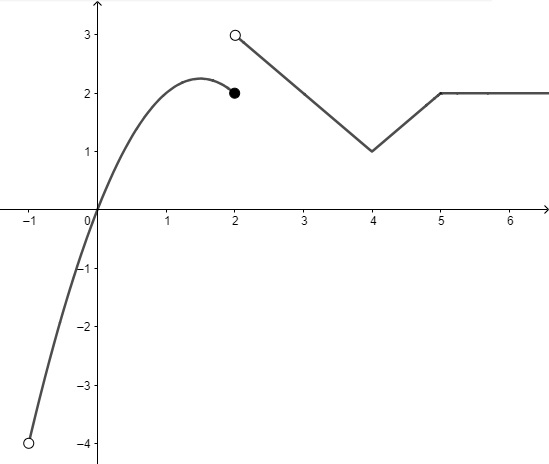
\includegraphics[width=3.8cm]{figures/funch.jpg}
\end{center}

Determine os intervalos de monotonicidade e os extremos de $h$.
\end{exemplo}
\end{frame}

%------------------------------------------------------------------------------------------------------------
\section{Atividade Online}
\begin{frame}
\frametitle{Atividade Online} %\framesubtitle{Exemplos}

\href{https://pt.khanacademy.org/math/algebra/algebra-functions/positive-negative-increasing-decreasing-intervals/e/increasing-decreasing-intervals-of-functions}
{{\tt Atividade 12 - Intervalos Crescentes e Decrescentes}}

\href{https://pt.khanacademy.org/math/algebra/algebra-functions/maximum-and-minimum-points/e/recognize-maxima-and-minima}
{{\tt Atividade 13 - Mínimos e Máximos Relativos}}

\href{https://pt.khanacademy.org/math/algebra/algebra-functions/maximum-and-minimum-points/e/recognize-absolute-maxima-and-minima}
{{\tt Atividade 14 - Mínimos e Máximos Absolutos}}

Veja o desempenho na Missão Álgebra I.


\end{frame}


%------------------------------------------------------------------------------------------------------------

\section{Exercícios}
\begin{frame}
\frametitle{Exercícios} %\framesubtitle{Exemplos}
\Ex{Considere a função $g: [0 ; 5] \to \R$ definida por: $$g(x) =
																\begin{cases}
																4x-x^2 & \ \text{ se } \ x< 3 \\
																x-2 & \ \text{ se } \  x \geq 3 \\
																\end{cases}.$$
Determine as soluções de:
\begin{enumerate}[(a)]
	\item $g(x) = -1$;
	\item $g(x) = 0$;
	\item $g(x) = 3$;
	\item $g(x) = 4$;
	\item $g(x) < 3$;
	\item $g(x) \geq 3$.
\end{enumerate} }
\end{frame}


%------------------------------------------------------------------------------------------------------------

\begin{frame}
\frametitle{Exercícios} %\framesubtitle{Exemplos}

\Ex{Sejam $f: \R \to \R $. Determine se as afirmações abaixo são
verdadeiras ou falsas, justificando suas respostas. As funções que
forem usadas como contraexemplo podem ser exibidas somente com o
esboço de seu gráfico.
\begin{enumerate}[(a)]
	\item Se $f$ é limitada superiormente, então $f$ tem pelo menos um máximo absoluto;
	\item Se $f$ é limitada superiormente, então $f$ tem pelo menos um máximo local;
	\item Se $f$ tem um máximo local, então $f$ tem um máximo absoluto;
	\item Todo máximo local de $f$ é máximo absoluto;
	\item Todo máximo absoluto de $f$ é máximo local;
	\item Se $x_0$ é o ponto de extremo local de $f$, então é ponto de
	extremo local de $f^2$, onde $(f^2)(x) = f(x) \cdot f(x)$;
	\item Se $x_0$ é o ponto de extremo local de $f^2$, então é ponto de
	extremo local de $f$.
\end{enumerate}}
\end{frame}


%------------------------------------------------------------------------------------------------------------

\begin{frame}
\frametitle{Exercícios} %\framesubtitle{Exemplos}

\Ex{Sejam $f: \R \to \R $ e $g: \R \to \R$. Determine se as
afirmações abaixo são verdadeiras ou falsas, justificando suas
respostas. As funções que forem usadas como contraexemplo podem ser
exibidas somente com o esboço de seu gráfico.
\begin{enumerate}[(a)]
	\item Se $f$ e $g$ são crescentes, então a composta $f \circ g$ é uma função crescente;
	\item Se $f$ e $g$ são crescentes, então o produto $f\cdot g$ é
	uma função crescente, onde $(f \cdot g)(x) = f(x) \cdot g(x)$;
	\item Se $f$ é crescente em $A \subset \R$ e em $B \subset \R$, então $f$ é crescente em $A \cup B \subset \R$.
\end{enumerate}}

\Ex{Mostre que a função inversa de uma função crescente é também uma
função crescente. E a função inversa de uma função decrescente é
decrescente.}

\end{frame}

%------------------------------------------------------------------------------------------------------------

\section{Bibliografia}

\frame{
	\frametitle{Bibliografia}
	\begin{thebibliography}{99}
		\bibitem {label1}
		IEZZI, Gelson; et al.
		\newblock \emph{Fundamentos de Matemática Elementar. Vol. 1 - Conjuntos e Funções}.
		\newblock São Paulo: Editora Atual.
	\end{thebibliography}
}

\end{document}
